
\documentclass[9pt,a5paper]{article}
\special{papersize=148mm,210mm}
\usepackage[left=2.2cm, right=1.5cm, top=1.5cm, bottom=1.5cm]{geometry}

\usepackage{graphicx}
\graphicspath{ {./} }

\usepackage[russian,english]{babel}
\usepackage[T2C]{fontenc}

\usepackage{array}
\usepackage{tabularx}
\usepackage{ragged2e}
\usepackage{amsmath}

\usepackage{multirow}

% Package for graphs
\usepackage{tikz}

% Package for letterspacing
\usepackage[letterspace=300]{microtype}

% \setdefaultlanguage{russian}

% For russian controls
\usepackage{amssymb}

\title{СИМПЛЕКТИЧЕСКИЕ МНОГООБРАЗИЯ}
\author{Илья Семенов}

\pagenumbering{gobble}

% Makes possible using vars
\makeatletter

% Document margins correction
\sloppy

% Add new table column styles
\newcolumntype{C}[1]{>{\centering\let\newline\\\arraybackslash\hspace{0pt}}m{#1}}
\newcolumntype{R}[1]{>{\RaggedLeft\arraybackslash}p{#1}}

\setlength{\tabcolsep}{0pt}
\renewcommand{\arraystretch}{1}

% Replace eng >= <= to rus ones
\renewcommand{\leq}{\leqslant}
\renewcommand{\geq}{\geqslant}
\renewcommand{\epsilon}{\varepsilon}
\renewcommand{\theta}{\vartheta}
\renewcommand{\phi}{\varphi}

% Макросы для векторного рисунка
\newcommand{\circlenode}{node[minimum size=2.2pt, inner sep=0pt, outer sep=0pt, draw, circle, fill=white] {}}
\newcommand\textnode[3]{node[minimum size=0pt, inner sep=0pt, outer sep=0pt, rotate=#2] {\scalebox{#3}{#1}}}
\newcommand\backgroundnode[3]{node[rotate=#3, fill=white, minimum width=#1, minimum height=#2] {}}

\newcommand\hs[1]{\hspace{#1}}
\newcommand\vs[1]{\vspace{#1}}
\newcommand\s[2]{\scalebox{#1}{#2}}

\newcommand\eq{\hs{-.6pt}=\joinrel\hs{-4pt}=\hs{-.6pt}}
\newcommand\eqv{\hs{-1pt}\equiv\joinrel\hs{-4pt}\equiv\hs{-1pt}}
\newcommand\rarrow{\hs{3pt}-\hs{-5pt}\joinrel\xrightarrow{}}
\newcommand\ti{-\joinrel\hs{-4pt}-}


% Remove space around align
\setlength{\abovedisplayskip}{0pt}
\setlength{\belowdisplayskip}{0pt}
\setlength{\abovedisplayshortskip}{0pt}
\setlength{\belowdisplayshortskip}{0pt}

% Set default latex font
\newcommand\Lcs[1]{{\normalfont\ttfamily\textbackslash#1}}

\begin{document}
\hs{-20pt}
\begin{tabularx}{\textwidth}{m{.2\textwidth} C{.6\textwidth} R{.2\textwidth}}
\footnotesize180& \s{.69}{\@title} & \s{.69}{[ГЛ.8}\hs{100pt}
\end{tabularx}

\vs{10pt}

\small\textbf{Д. Условие коммутативности потоков.} Пусть $\pmb{A}, \hs{5pt} \pmb{B}$ --- векторные поля \hs{2pt} на \hs{1pt} многообразии \hs{2pt} $M$.

\vs{-1pt}

\small\textls{Теорема}\hs{-1pt}. \hs{.5pt} \textit{Два потока \hs{1pt} $A^{t}, \hs{2pt} B^{s}$ \hs{1pt} коммутируют \hs{1pt} тогда \hs{1pt} и 
\hs{1pt} только \newline тогда, \hs{2pt} когда \hs{2pt} скобка \hs{4pt} Пуассона \hs{2pt} соответствующих \hs{1pt} векторных \hs{1pt} полей \newline $\pmb{[A,\hs{8pt} B]}$ \hs{.5pt} равна \hs{.5pt} нулю.}

\vs{-1.5pt}

\small\textls{Доказательство}\hs{-1pt}.\hs{5pt} Если \hs{7pt} $A^{t} B^{s} \eqv B^{s}A^{t}$, \hs{3pt} то \hs{4pt} по \hs{4pt} лемме \hs{6pt}1 \newline 
$\pmb{[A, \hs{10pt} B]} \eq 0$.
\hs{3pt} Если \hs{2pt} $\pmb{[A,\hs{5pt} B]} = 0$, \hs{2pt} то по \hs{1pt} лемме \hs{.7pt} 1 \hs{0pt} для \hs{1pt} любой \hs{1pt}функции \newline $\phi$ \hs{2pt} в \hs{0pt} любой \hs{1pt} точке \textit{x}
\vs{-6pt}
\[
\phi(A^{t}B^{s}x) \hs{2pt} \text{---} \hs{2pt} \phi(B^{s}A^{t}x) \eq o(s^2+t^2), \quad s \rarrow 0, t \rarrow 0. \vs{-3.5pt}
\]
Мы \hs{1pt} покажем, \hs{1pt} что отсюда \hs{1pt} вытекает \hs{1pt} $\phi(A^{t}B^{s}x) \eq \phi(B^{s}A^{t}x)$ \hs{1pt} при доста- \newline точно \hs{1pt} малых \hs{1pt} $s$ \hs{.2pt} и \hs{0pt} $t$.

\vs{5pt}

\footnotesize \hs{1pt} Применяя это соотношение к \hs{1pt} локальным координатам $(\phi \eq x_1,\,\dots,\,\phi \eq x_n)$, \vs{-11pt}\newline
получим $A^{t}B^{s} \eqv B^{s}A^{t}$.

\vs{-2pt}

\footnotesize \hs{1pt} Рассомтрим прямоугольник \hs{1pt} $0 \hs{1pt} \leq \hs{1pt} t \hs{1pt} \leq \hs{1pt} t_0$, $0 \leq s \leq s_0$ \hs{.2pt} (рис. 170) на плоскости \vs{-1pt}\newline 
$(t, \hs{2pt} s)$. \hs{-2pt} Каждому пути, \hs{0pt} ведущему \hs{-3pt} из $(0, \hs{2pt} 0)$ \hs{1pt} в $(t_0, s_0)$ и состоящему \hs{1pt} из конечного \vs{-1pt}\newline
числа \hs{.5pt} отрезков координатных направлений, сопоставим произведение преобра- \newline
зований \hs{1pt} потоков \hs{1pt} $A^{t}$ \hs{1pt} и \hs{.5pt} $B^{s}$. Каждому отрезку $t_1 \hs{.5pt}\leq\hs{.5pt} l \hs{.5pt}\leq\hs{.5pt} t_2$ \hs{.5pt} сопоставим $A^{t_2-t_1}$,

\hs{-18pt}
\begin{tabular}{m{5.1cm} c}
        & \multirow{2}{*}{
            \begin{tikzpicture}[scale=1.35, transform shape]
                % Внешняя фигура
                \draw 
                    (0,0) to[out=168,in=10] 
                    (-2.5,.05) to[out=79,in=-60] 
                    (-2.86,2.61) to[out=18.5,in=158] 
                    (.4,2.7) to[out=-92,in=75] (0,0);
        
                % Внутренняя фигура
                \draw  
                    (.03,1.98) \circlenode to[out=-100,in=70] 
                    (-.42,.42) \circlenode to[out=172,in=4] 
                    (-1.96,.56) \circlenode to[out=95,in=-65] 
                    (-2.29,2.33) \circlenode to[out=25,in=177] 
                    (-.51,2.595) \circlenode;
    
                % Внутренная фигура 2
                \draw 
                    (-1.16,1.45) -- 
                    (-1.095,1.78) \circlenode  -- 
                    (-.83,1.735) \circlenode -- 
                    (-.75,2.04) -- 
                    (-.52,2) -- 
                    (-.48,2.21) \circlenode;
    
                % Внутренная фигура 3
                \draw 
                    (-1.45,.55) to[out=88,in=-90] 
                    (-1.42,1.46) to[out=5,in=177] 
                    (-1.16,1.45) \circlenode to[out=3,in=170] 
                    (-.8,1.39) \circlenode -- 
                    (-.71,1.71) \circlenode -- 
                    (-.65,1.95) -- 
                    (-.43,1.91) -- 
                    (-.37,2.17) \circlenode;
    
                % Текстовые подписи
                \draw 
                    (.5,1.9) \backgroundnode{20pt}{7.5pt}{5}
                    (.13,1.85) \textnode{$B$}{5}{.7}
                    (.25,1.98) \textnode{$s$}{5}{.7}
                    (.33,1.91) \textnode{$0$}{-10}{.42}
                    (.39,1.88) \textnode{$A$}{5}{.7}
                    (.51,1.98) \textnode{$t$}{5}{.6}
                    (.59,1.93) \textnode{$0$}{-10}{.42}
                    (.7,1.89) \textnode{$x$}{5}{.7}
                    
                    (-.55,.28) \textnode{$A$}{-22}{.6}
                    (-.4,.32) \textnode{$t$}{-22}{.7}
                    (-.34,.24) \textnode{0}{-32}{.4}
                    (-.24,.18) \textnode{$x$}{-22}{.7}
    
                    (-2.13,.36) \textnode{\textit{M}}{0}{.7}
                    (-1.85,.36) \textnode{$x$}{0}{.7}
    
                    (-2.55,2.49) \textnode{$B$}{0}{.7}
                    (-2.39,2.62) \textnode{$s$}{0}{.72}
                    (-2.3,2.55) \textnode{$0$}{-10}{.4}
                    (-2.2,2.5) \textnode{$x$}{10}{.7}
    
                    (-.83,2.8) \textnode{$A$}{-10}{.7}
                    (-.68,2.88) \textnode{$t$}{-10}{.65}
                    (-.62,2.81) \textnode{$0$}{-20}{.42}
                    (-.53,2.75) \textnode{$B$}{-15}{.7}
                    (-.35,2.85) \textnode{$s$}{-15}{.7}
                    (-.28,2.78) \textnode{$0$}{-30}{.42}
                    (-.2,2.70) \textnode{$x$}{-15}{.7}
    
                    (-.2,2.14) \textnode{$\beta'$}{0}{.7}
                    (-.58,1.65) \textnode{$\beta$}{0}{.7}
                    (-.8,1.23) \textnode{$\gamma$}{0}{.8}
                    (-1.21,1.29) \textnode{$\delta$}{0}{.7}
                    (-1.22,1.78) \textnode{$\epsilon$}{0}{.7}
                    (-.92,1.9) \textnode{$\alpha$}{0}{.7}
                    (-.63,2.33) \textnode{$\alpha'$}{0}{.7};
            \end{tikzpicture}
        }\\[-18pt]
        \vs{10pt}
         отрезку \hs{2pt} $s_1 \hs{.5pt}\leq\hs{.5pt} s \hs{.5pt}\leq\hs{.5pt} s_2 - B^{s_2-s_1}$; при- \vs{-1pt}\newline 
         менять \hs{2pt} преобразования \hs{2pt} будем \hs{2.4pt} в \vs{-1pt}\newline
         порядке, \hs{1.1pt} в \hs{1pt} каком идут отрезки от \vs{-1pt}\newline
         $(0, \hs{3pt} 0)$.
     &         

    \\[18pt]
        \centering
        \hs{-6pt}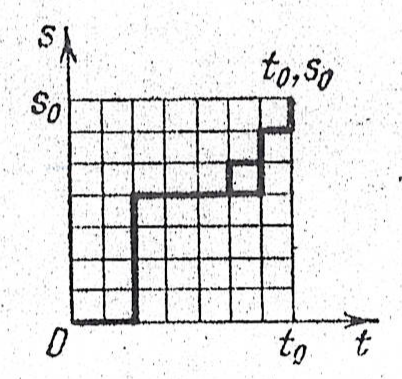
\includegraphics[scale=.24]{pic1}\hs{1pt}
    &\\
    \centering\scriptsize Рис. \hs{1.5pt} 170. \hs{0pt} К доказатель- & \scriptsize Рис. \hs{2pt} 171. \hs{2pt} Криволинейный четырех- \\[-3pt]
    \centering\scriptsize ству коммутативности & \scriptsize угольник $\beta\gamma\delta\epsilon\alpha$. \\[-3pt]
    \centering\scriptsize потоков. &
\end{tabular}

\vs{7pt}

\footnotesize \hs{.5pt} Так, например, \hs{1pt} сторонам \hs{1pt} $(0 \hs{.5pt}\leq\hs{.5pt} t \hs{.5pt}\leq\hs{.5pt} t_0, s \eq 0)$ и \hs{1pt} $(t \eq t_0, 0 \hs{.5pt}\leq\hs{.5pt} s \hs{.5pt}\leq\hs{.5pt} s_0)$ отвечает \newline
произведение \hs{1pt} $B^{s_0}A^{t_0}$, а сторонам \hs{1pt} $(t \eq 0, 0 \hs{.5pt}\leq\hs{.5pt} s \hs{.5pt}\leq\hs{.5pt} s_0)$ \hs{3pt} и \hs{2pt} $(s \eq s_0, 0 \hs{.5pt}\leq\hs{.5pt} t \hs{.5pt}\leq\hs{.5} t_0)$ --- \newline
произведение $A^{t_0}B^{s_0}$.

\vs{.5pt}

\footnotesize \hs{.5pt} Кроме того, мы сопоставим каждому \hs{1pt} такому пути на \hs{1pt} плоскости \hs{0pt} $(t, \hs{2pt} s)$ путь \newline
\hs{1pt} на \hs{1pt} монгообразии \hs{1pt} $M$, \hs{1pt} выходящий \hs{.6pt} из \hs{.59pt} точти \hs{.8pt} \textit{x}, \hs{1pt} составленный \hs{1pt} из \hs{.2pt} траекторий \vs{-1pt} \newline
потоков \hs{1pt} $A^{t}$ \hs{.8pt} и \hs{.8pt} $B^{s}$ \hs{.1pt} (рис. 171). \hs{1pt} Если \hs{1pt} пути \hs{1pt} на плоскости \hs{1pt} $(t, \hs{2pt} s)$ \hs{.5pt} соответствует \vs{2pt} \newline
преобразование $A^{t_1}B^{s_1} \dots A^{t_n}B^{s_n}$, то на монгообразии $M$ соответствующий путь \vs{-7pt}\newline
заканчивается \hs{.5pt} в точке \hs{-.8pt} $A^{t_1}B^{s_1} \dots A^{t_n}B^{s_n}$\textit{x}.

\hs{.5pt} Наша цель --- доказать, что все эти пути в действительности заканчиваются \newline
в одной точке $A^{t_0}B^{s_0} \eq A^{t_0}B^{s_0}$\textit{x}.

\hs{.5pt} Разобъем отрезки $(0 \hs{.5pt}\leq\hs{.5pt} t \hs{.5pt}\leq\hs{.5pt} t_0)$ и $(0 \hs{.5pt}\leq\hs{.5pt} s \hs{.5pt}\leq\hs{.5pt} s_0)$ на \hs{1pt} $N$ равных частей так, \hs{1pt} что \vs{-1pt}\newline
весь \hs{1pt} прямоугольник \hs{1pt} разделится на $N^2$ \hs{.5pt} маленьких прямоугольников. Переход \vs{-1pt}\newline
от \hs{1pt} сторон $(0, \hs{2pt} 0)$ --- $(0, \hs{2pt} t_0)$ --- $(s_0, \hs{2pt} t_0)$ к сторонам $(0, \hs{2pt} 0)$ --- $(s_0, \hs{2pt} 0)$ --- $(s_0, \hs{2pt} t_0)$ можно \vs{-1pt}\newline
совершить \hs{.5pt} в \hs{1pt} $N^2$ шагов, \hs{1pt} в каждом из которых \hs{1pt} пара соведних сторон малень- \vs{-1pt}\newline
кого прямоугольника \hs{1pt} заменяется другой парой \hs{1pt} (рис. 172).
\end{document}
